\documentclass[11pt, ngerman, fleqn, DIV=15, headinclude, BCOR=2cm]{scrreprt}

\usepackage{../../header}

\usepackage[section]{placeins}
\usepackage[maxfloats=50]{morefloats}
\usepackage{subcaption}

\usepackage{csquotes}


\usepackage{tikz}
\usetikzlibrary{chains}
\usetikzlibrary{shapes.geometric}

\tikzset{device/.style={
                rectangle,
                minimum size=6mm,
                draw=black
            },
            monitor/.style={
                rectangle,
                rounded corners=2mm,
                minimum size=6mm,
                draw=black
            },
        }

\usepackage{pgfplots}
\pgfplotsset{
    compat=1.9,
    width=0.8\linewidth,
    xticklabel style={/pgf/number format/use comma},
    yticklabel style={/pgf/number format/use comma},
}
\usepgfplotslibrary{polar}

\usepgfplotslibrary{external}
\tikzexternalize[mode=list and make]
\tikzsetexternalprefix{Abbildung-}

\DeclareSIUnit{\skt}{SKT}

\usepackage{booktabs}

\hypersetup{
    pdftitle=
}

\newcommand{\plotwidth}{0.8\linewidth}

\subject{Praktikumsprotokoll}
\title{$\gamma$-Spektroskopie mit Szintillations- und Halbleiterdetektoren}
\subtitle{Versuch P521 -- Universität Bonn}
\author{
	Frederike Schrödel \\
	\small{\href{mailto:fschroedel@gmx.de}{fschroedel@gmx.de}}
	\and
	Simon Schlepphorst \\
	\small{\href{mailto:s2@uni-bonn.de}{s2@uni-bonn.de}}
}

\date{2015-11-09 bis 11-12}

\publishers{Tutor: Philipp Hoffmeister
}

\begin{document}

\maketitle

\begin{abstract}
    In diesen Versuch geht es darum, die Eigenschaften von einem
    Szintillationsdetektor und einem Ge-Halbleiterdetektor bei der
    $\gamma$-Spektroskopie zu vergleichen.
    Dabei sind die Energieauflösung und die Nachweiswahrscheinlichkeit die
    zu untersuchenden Eigenschaften.
\end{abstract}


\tableofcontents

\chapter{Theorie}

\section{Wechselwirkung von $\gamma$-Strahlung mit Materie}
Die $\gamma$-Strahlung entsteht wenn nach einem vorhergegangen Zerfall der
Tochterkern nicht in seinen Grundzustand, sondern in einen angeregten Zustand
zerfällt.
Dieser angeregte Zustand zerfällt nach einiger Zeit durch Abstrahlung des
$\gamma$-Quants in den Grundzustand. Die Photonen sind sehr energiereich,
weshalb sie genug Energie haben, um auf verschiedene Weisen mit der Materie zu
wechselwirken.
Die Art der Wechselwirkung hängt dabei von der Ordnungszahl der bestrahlten Atome
und der Energie der $\gamma$-Strahlung ab.

\subsection{Photoeffekt}
Der Photoeffekt beschreibt den Vorgang, bei dem ein Photon ein Elektron aus
dem Atom auslöst.
Hierbei gibt das Photon seine komplette Energie ab.
Die kinetische Energie des ausgelösten Elektrons hängt nur mit der
Bindungsenergie ($E_\text{Bind.}$) und der Energie des Photons ($h\nu$),
also dessen Frequenz ($\nu$), zusammen.
\[ 
    E = h\nu - E_\text{Bind.}
\]
Wenn man sich den Wirkungsquerschnitt $\sigma$ für den Prozess anschaut,
dann stellt man eine große Abhängigkeit von der Ordnungszahl $Z$ fest.
\[
    \sigma \propto Z^5 E_\gamma^{\frac 72}
\]
Deshalb tritt dieser Effekt besonders häufig bei Elementen mit hoher Ordnungszahl
auf.

\subsection{Paarerzeugung}

Ein anderer Effekt, der bei Energien $E_\gamma \ge 2m_\text ec^2$ auftreten
kann, ist die Elektron-Positron-Paarbildung. Wenn ein Photon ausreichend
Energie hat, so kann es ein Elektron-Positron-Paar bilden. Die Energie, die das
Photon über die Ruhemassen der beiden Teilchen hinaus hatte, bekommen diese in
Form von kinetischer Energie. Diese Energie können sie über Stöße abgeben.
Sobald das Positron keine kinetische Energie mehr hat, kann es mit einem
Elektron unter Abstrahlung von zwei Photonen mit \SI{511}{\kilo\electronvolt}
und entgegengesetzter Bewegungsrichtung annihilieren. Dieser Prozess kann nur in der Nähe eines Atomkerns stattfinden weil dieser
den Rückstoß aufnehmen muss.
Dadurch bleibt bei diesen Vorgang Energie und Impuls erhalten.

Ausschlag gebend ist der Effekt allerdings erst weit oberhalb dieser Schwelle.
Für den Wirkungsquerschnitt gilt $\sigma \propto Z^2$.

\subsection{Comptonstreuung}
Wenn Photonen an einem Elektron streuen, spricht man vom Comptoneffekt. 
Hierbei gibt das Photon einen Teil seiner Energie an das Elektron ab und ändert dabei
die eigene Frequenz.
Die abgegebene Energie hängt vom Streuwinkel ab.
Für die Restenergie des Photons gilt:
\[
    E_\nu'(\phi) = \frac{E_\nu}{1+\frac{E_\nu}{m_\text ec^2}(1+\cos(\phi))}
\]
Die größte Energieänderung erhält man also bei einem Winkel von
$\phi=\SI{180}{\degree}$.
Diese Energieänderung berechnet sich durch:
\[
    \delta\lambda = \frac{h}{m_\text ec}(1-\cos(\phi))
\]
Der Wirkungsquerschnitt entspricht $\sigma_\text C \propto \frac{Z}{E_\gamma}$.

\subsection{Keine Wechselwirkung}
Ein nicht unerheblicher Teil der $\gamma$-Strahlung kann auch ohne Wechselwirkung
Materie durchdringen.

\section{Szintillationsdetektor}

Mit einem Szintillationsdetektor lassen sich Intensität und Energie von
ionisierender Strahlung messen.
Er besteht aus einem Szintillator und einem Photomultiplier.
Der Szintillator ist ein dotierter Einkristall, der von energiereicher
Strahlung zum Fluoreszieren angeregt werden kann und hinreichend
durchlässig für das von ihm emittierte Licht ist.

Innerhalb des vor Lichteinfall geschützten Szintillators entstehen durch
ionisierende Strahlung Lichtblitze. 
Wie viele dieser Blitze auftreten ist von der Energie der Strahlung abhängig.
Durch den Photoeffekt werden an der Photokathode des Photomultipliers
Elektronen ausgelöst.
Es kommt innerhalb des Photomultiplieres zu einem Lawineneffekt,
der die Elektronen vervielfacht und somit ein Signal verstärkt.
Die Amplitude des entstanden Strompulses ist somit auch proportional zu der
Energie der Eingangsstrahlung.

Wenn man eine gute Energieauflösung möchte, ist diese Detektorart nicht
besonders geeignet. Hier empfiehlt es sich einen Halbleiterdetektor zu
verwenden. Dieser ist dafür deutlich besser geeignet ist, wie im weiteren Verlauf noch
deutlich wird.

% TODO Und warum sollte man das?

\section{Halbleiterdetektor}

Die Basis des Halbleiterdetektors bildet die Verarmungszone, die zwischen einem
$p$- und einem $n$-dotierten Halbleiter entsteht.

Betrachtet man das Bändermodel von Halbleitern, so kann man sich die Dotierung
des Halbleiters als weiteres dünnes Band knapp unter dem Leitungsband
($n$-dotiert) oder knapp über dem Valenzband ($p$-dotiert) vorstellen.
Man erhält die Dotierung eines Kristalls, indem man fremde Atome in den
Kristall einbindet.
Wenn man eine positive Dotierung möchte, so fügt man in den Kristall Atome mit
einer niedrigeren Anzahl Valenzelektronen ein, für die negative Dotierung nutzt
man Atome mit höherer Valenzelektronenanzahl.

Fügt man diese beiden Bereiche aneinander, so entsteht dazwischen eine Bereich,
indem die überschüssigen Elektronen aus dem $n$-dotierten Teil in den
$p$-dotierten Bereich übergehen.
Hierdurch bildet sich durch die zurückbleibenden Ionenrümpfe ein elektrisches Feld aus, welches
der weitern Verbreiterung der Verarmungszone entgegen wirkt.
Es entspricht somit einer Diode.
Wenn man diese nun in Sperrrichtung betreibt, kann man die Verarmungszone weiter
verbreitern.
Das ist erwünscht, da nur in diesen Bereich des Detektors Ereignisse
gemessen werden können.
Wenn ein $\gamma$-Quant innerhalb der Verarmungszone  ein Elektronen-Loch-Paar
erzeugt, werden diese zu den Seiten hin abgesaugt und ergeben das Signal.

\subsection{Multi-Channel-Analyzer}

Um ein nach Amplituden sortiertes Spektrum zu erhalten, nutzen wir ein MCA.
Es ist ein Bauteil, dass einkommende Signale nach Amplitude sortiert und
dann den entsprechenden Kanal hoch zählt. So erhalten wir ein
Histogramm.

%TODO Bild Spektrum
%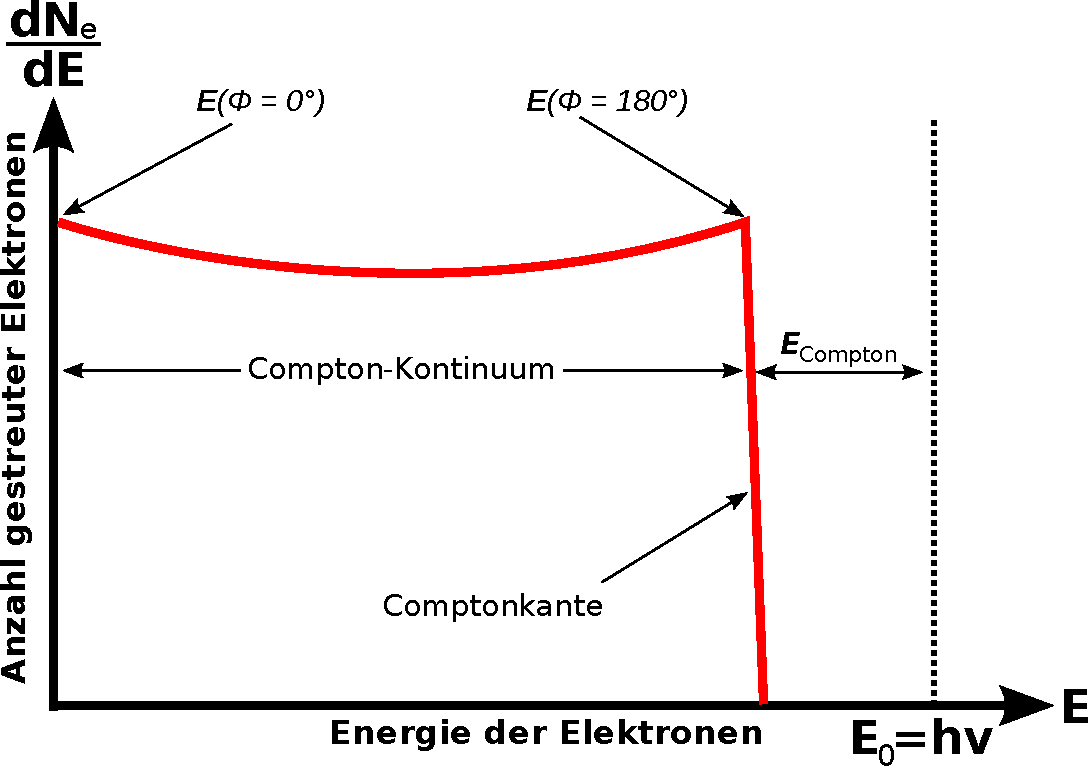
\includegraphics[width=0.5\linewidth]{../graphics/Compton-spektrum.pdf}
%\parencite{comptoneffekt}

%In dem schematischen Spektrum, erkennt man ein Compton-Kontinuum, welches die 
%Comptonstreuung bis zu einem Winkel von \SI{180}{\degree} enthält. Da bei diesem
%Wert der maximale Energieübertrag stattfindet, erhält man die scharfe Compton Kante.
%Wird nicht nur ein Teil sondern die gesamte Energie abgegeben, wie es beim
%Photoeffekt der Fall ist, entsteht der energetisch höher gelegene Ausschlag. Man 
%nennt ihn Photo-Peak.

\chapter{Aufbau und Durchführung}

Der Aufbau des Experiments sieht wie folgt aus:

Die Detektoren sind an einen Signalverstärker angeschlossen, der
wiederum an einen Vielkanalanalysator angeschlossen ist.

Für die Durchführung müssen zunächst die Betriebsparameter wie die
Verstärkung des Signalverstärkers eingestellt werden.
Dazu werden die Proben jeweils einzeln vor die Detektoren gestellt und das
Ausgangssignal des Signalverstärkers am Oszilloskop betrachtet.
Die Verstärkung ist so eingestellt, dass die für die Energiekalibrierung
wichtige \SI{1408}{\kilo\electronvolt}-Linie des $^{152}\text{Eu}$
innerhalb des Messbereichs liegt.
%TODO Foto vom Aufbau

Nun messen wir mit beiden Detektoren für alle drei Proben, $^{60}\text{Co}$,
$^{137}\text{Cs}$ und $^{152}\text{Eu}$, und den Untergrund jeweils ein
Spektrum. Jede dieser Messungen wird über einen Zeitraum von fünf Minuten aufgenommen.

Für die Langzeitmessung mit dem Ge-Detektor wird eine Bleiabschirmung
aufgebaut, mit der über Nacht der Untergrund gemessen wird, bevor die Bodenprobe
innerhalb der Abschirmung positioniert wird und erneut über Nacht gemessen wird.

\chapter{Kalibrierungen}

\section{Vorbereitungen}

Bevor wir anfangen können die Spektren zu untersuchen, müssen zunächst die
Aufnahmezeiten angepasst werden, da wir die Realzeit auf \SI{600}{\second} gesetzt
haben und diese durch Totzeiten des Detektors von der Aufnahmezeit abweicht.
Nach Anpassung der Zeit müssen wir die Untergrundmessung von der Messung der Spektren 
abziehen. Von den gefilterten Spektren untersuchen wir im folgenden die durch
$\gamma$-Zerfall entstandenen Ausschläge, wie in
Abbildung~\ref{fig:energiekalibrierung} zu sehen ist.
% FIXME Satzende?

\begin{figure}[htbp]
    \centering
    \includegraphics[width=\plotwidth]{Ge_calib}
    \caption{%
	    $^{152}\text{Eu}$-Spektrum im Ge-Detektor
        %
    }
    \label{fig:energiekalibrierung}
\end{figure}

\section{Spektren}
\subsection{Szintillationsspektrometer}

\begin{figure}[htbp]
	\centering
	\includegraphics[width=\plotwidth]{Sz_CS}
	\caption{%
            Szintillationsspektrometer mit $^{137}\text{Cs}$-Quelle
	}
	\label{fig:}
\end{figure}
\begin{figure}[htbp]
	\centering
	\includegraphics[width=\plotwidth]{Sz_CO}
	\caption{%
            Szintillationsspektrometer mit $^{60}\text{Co}$-Quelle
	}
	\label{fig:}
\end{figure}
\begin{figure}[htbp]
	\centering
	\includegraphics[width=\plotwidth]{Sz_EU}
	\caption{%
            Szintillationsspektrometer mit $^{152}\text{Eu}$-Quelle
	}
	\label{fig:}
\end{figure}


\subsection{Ge-Detektor}

\begin{figure}[htbp]
	\centering
	\includegraphics[width=\plotwidth]{Ge_CS}
	\caption{%
            Ge-Detektor mit $^{137}\text{Cs}$-Quelle
	}
	\label{fig:}
\end{figure}
\begin{figure}[htbp]
	\centering
	\includegraphics[width=\plotwidth]{Ge_CO}
	\caption{%
            Ge-Detektor mit $^{60}\text{Co}$-Quelle
	}
	\label{fig:}
\end{figure}
\begin{figure}[htbp]
	\centering
	\includegraphics[width=\plotwidth]{Ge_EU}
	\caption{%
            Ge-Detektor mit $^{152}\text{Eu}$-Quelle
	}
	\label{fig:}
\end{figure}




\section{Energiekalibrierung}

Weil die Spektren mit einem Vielkanalanalysator aufgenommen werden, muss eine
Energiekalibrierung vorgenommen werden. Hierbei wird den Nummern der 8192
Kanäle die Energie zugeordnet der sie entsprechen.
Das erreichen wir indem wir an Ausschläge bekannter $\gamma$-Übergänge
Verteilungsfunktionen anpassen. Über den Schwerpunkt erhalten wir die Kanalnummer zu 
der vorgegebenen Energie . 
An die Daten aus dem NaJ(Ti)-Detektor haben wir Gaußkurven und an die
aus dem Ge-Detektor Lorentzkurven angepasst, da diese näher an den Daten liegen.
Somit wurde den Kanalnummern eine Energie zugeordnet. Das ist in
Abbildung~\ref{fig:Ge-peaks} zu sehen.
% FIXME Satzende?

\begin{tabular}{SSSSSS}
    {Nummer} & {Kanal} & {Breite $\Gamma$} & {Fläche} & {rel.\ Intens.} &
    {$E_\gamma$ / \si{\kilo\electronvolt}} \\
    \midrule
    %< for row in sz_fits_table >%
    << ' & '.join(row) >> \\
    %< endfor >%
\end{tabular}

Für den NaJ(Ti)-Detektor nutzen wir die beiden am besten getrennten Linien des
$^{152}\text{Eu}$: die Linie des $^{137}\text{Cs}$ und die Linien des
$^{60}\text{Co}$.

\begin{tabular}{SSSSSS}
    {Nummer} & {Kanal} & {Breite $\Gamma$} & {Fläche} & {rel.\ Intens.} &
    {$E_\gamma$ / \si{\kilo\electronvolt}} \\
    \midrule
    %< for row in ge_eu_fits_table >%
    << ' & '.join(row) >> \\
    %< endfor >%
    \midrule
    %< for row in ge_cs_fits_table >%
    << ' & '.join(row) >> \\
    %< endfor >%
    \midrule
    %< for row in ge_co_fits_table >%
    << ' & '.join(row) >> \\
    %< endfor >%
\end{tabular}

Da die Energieauflösung des Ge-Detektors deutlich besser ist als die des 
NaJ(Ti)-Detektors lassen sich deutlich mehr Linien des $^{152}\text{Eu}$
erkennen und trennen sodass wir davon sieben verwerten konnten.

Das Energie-zu-Kanal Verhältnis haben wir grafisch in
Abbildung~\ref{fig:ge_kanal} für den
Ge-Detektor und in Abbildung~\ref{fig:sz_kanal} für den NaJ(Ti)-Detektor aufgetragen.
Die angepassten Geraden haben folgende Werte:

NaJ(Ti)-Detektor
\[
    \text{Energie} =
    \text{Kanalnummer} \cdot \SI{<< sz_slope >>}{\kilo\electronvolt}
    +
    \SI{<< sz_offset >>}{\kilo\electronvolt} \,.
\]
Ge-Detektor
\[
    \text{Energie} =
    \text{Kanalnummer} \cdot \SI{<< ge_slope >>}{\kilo\electronvolt}
    +
    \SI{<< ge_offset >>}{\kilo\electronvolt} \,.
\]

\section{Halbwertsbreiten}
Da wir bereits Lorentz- und Gaußkurven angepasst haben um den Schwerpunkt zu
bestimmen, kennen wir auch die Halbwertsbreiten $\Gamma$.

\begin{align*}
	f_\text{Gauß}\del x &= \frac1{\sigma \sqrt{2\pi}}
	\eup^{-\frac12\del{\frac{x
	- \langle x\rangle}{\sigma}}^2}
	&&\text{mit FWHM} = 2.35\sigma\\
	\\
	f_\text{Lorentz}\del x &= \frac1\pi \frac\sigma{\del{x - \langle x
	\rangle}^2 + \sigma^2}
	&&\text{mit FWHM} = \sigma\\
\end{align*}

%TODO kommentar zur detektor abhängigkeit.
An der Breite der Linien zeigt sich, um wie viel besser die Energieauflösung des
Ge-Detektors ist. Deshalb lassen sich mit dem Ge-Detektor mehr Linien
deutlich trennen.

\section{Intrinsische Halbwertbreite des Ge-Detektors}
Aus den Halbwertsbreiten der Linien, die mit dem Ge-Detektor aufgenommen
wurden,
lässt sich die intrinsische Halbwertsbreite $\Delta E_d$ bestimmen.
\[
	\Delta E_d(E_\gamma)=\text{Const}\cdot\sqrt{E_\gamma}
\]
Dieser Zusammenhang wurde in Abbildung~\ref{fig:halbwertsbreite} untersucht und die Konstante
ermittelt.
Mit dem Wert, den wir für die intrinsische Halbwertsbreite gefunden haben, lässt
sich wie folgt der elektronische Anteil der Halbwertsbreite bestimmen.
\[
	\Delta E(E_\gamma)=\sqrt{\Delta E_d(E_\gamma))^2+(\Delta E_e)^2}
\]
Wir erhalten:
\[
    \text{Const} = \num{<< ge_const >>}\,\sqrt{\si{\kilo\electronvolt}}
    ,\qquad
    \Delta E_\mathrm e = \SI{<< ge_electronic_width >>}{\kilo\electronvolt}
\]

\section{Nachweißgüte der Detektoren}

Nun soll das Verhältnis der Ereignisse im Photopeak gegenüber allen Ereignissen
im Detektor gebildet werden (Peak-to-Total-Verhältnis). Dies wird mit dem
Einzelpeak von $^{137}\text{Cs}$ und dem Summe aus dem Doppelpeak von
$^{60}\text{Co}$ durchgeführt:

NaJ(Ti)-Detektor
\[
    \text{Peak-to-Total (Cs, \SI{662}{\kilo\electronvolt})} = \num{<< sz_cs_ptt >>}
\]
\[
    \text{Peak-to-Total (Co, \SI{1250}{\kilo\electronvolt})} = \num{<< sz_co_ptt >>}
\]
Ge-Detektor
\[
    \text{Peak-to-Total (Cs, \SI{662}{\kilo\electronvolt})} = \num{<< ge_cs_ptt >>}
\]
\[
    \text{Peak-to-Total (Co, \SI{1250}{\kilo\electronvolt})} = \num{<< ge_co_ptt >>}
\]


Die absolute Peakeffizienz wird aus dem Verhältnis der Ereignisse im Photopeak
und aller ausgestrahlten $\gamma$-Quanten der Probe gebildet. Dazu benutzen wir
die bekannten Werte der $^{137}\text{Cs}$ Probe (\SI{0.925}{\mega\becquerel},
April 1985). Daraus erhalten wir eine aktuelle Aktivität von:
\[
	A\del{^{137}\text{Cs}} = \SI{<< cs_activity >>}{\becquerel}
\]
Bei einem Abstand von etwa \SI{25}{\centi\metre} zwischen Detektor und Probe
erhalten wir:

NaJ(Ti)-Detektor
\[
    \text{Absolute Peakeffizienz (Cs)} = \num{<< ge_cs_abs >>}
\]
Ge-Detektor
\[
    \text{Absolute Peakeffizienz (Cs)} = \num{<< sz_cs_abs >>}
\]


Um die relative Effizienz des Ge-Detektors zu bestimmen ermitteln wir die
relative Intensität aus der Fläche und der Energie der verschiedenen
$^{152}\text{Eu}$ Linien und normieren diese auf eine relative Intensität der
\SI{1408}{\kilo\electronvolt} Linie von 1000.
In Abbildung~\ref{fig:effizienz} ist die relative Effizienz aufgetragen, indem
wir die ermittelten relativen Intensitäten durch die erwarteten relativen
Intensitäten der $\gamma$-Linien geteilt haben.

\begin{tabular}{SSSS}
    {Energie / \si{\kilo\electronvolt}} & {rel.\ Intens. erw.} & {rel.\ Intens.
mess.} & {Effizienz} \\
    \midrule
    %< for row in ge_efficiency_table >%
    << ' & '.join(row) >> \\
    %< endfor >%
\end{tabular}

\begin{figure}
    \centering
    \includegraphics[width=\plotwidth]{halbwertsbreite_ge}
    \caption{%
	    Halbwertsbreite abhängig von der Energie im Ge-Detektor
        %
    }
    \label{fig:halbwertsbreite}
\end{figure}


\begin{figure}
    \centering
    \includegraphics[width=\plotwidth]{ge_efficiency}
    \caption{%
	    Energieabhängige Effizenz des Ge-Detektors.
        %
            Fit mit $a \cdot (E/\si{\kilo\electronvolt})^b + c$ mit
            $a = \num{<< ge_effizienz_a >>}$,
            $b = \num{<< ge_effizienz_b >>}$ und
            $c = \num{<< ge_effizienz_c >>}$.
    }
    \label{fig:effizienz}
\end{figure}






\clearpage
\chapter{Auswertung der Langzeitmessung}

\section{Vorbereitung des Spektrums}

Bei dem Vergleich von Daten und Untergrund aus der Langzeitmessung fällt sehr
schnell auf, dass der Untergrund deutlich höher liegt, als die Daten. Deshalb
ist es nicht möglich den Untergrund von den Daten abzuziehen um ein sauberes
Spektrum zu erhalten.

Stattdessen teilen wir alle Messwerte durch die vorher bestimme
Detektorgenauigkeit und können so den exponentiellen Abfall im Untergrund
herausfiltern. Da die Detektorgenauigkeit aber nur oberhalb von
\SI{200}{\kilo\electronvolt} damit genähert werden kann, beschränken wir uns in
der folgenden Auswertung ebenfalls auf diesen Bereich. Die so bereinigten
Spektren sind in Abbildung~\ref{fig:langzeit_probe_untergrund} zu sehen.

\begin{figure}
	\centering
	\includegraphics[width=\plotwidth]{plot_spektren_langzeit}
	\caption{%
		Vergleich von Proben- und Untergrundspektrum
	}
	\label{fig:langzeit_probe_untergrund}
\end{figure}

Die in diesem Spektrum von Hand identifizierten Linien haben wir dann einzeln
mit Lorentzkurven angepasst. Dies ist etwas unübersichtlich in
Abbildung~\ref{fig:langzeit_probe_peaks} dargestellt. Im Detail kann man die
einzelnen Anpassungen in Anhang~\ref{anhang-bodenprobe} betrachten. Dort sind
auch die Details der in Kapiten~\ref{identifizieren-isotope} beschriebenden
Auswertungsmethode zu sehen.
Die Ergebnisse sind dann in übersichtlicher Form in
Tabelle~\ref{tab:langzeit-anpassungen-tabelle} zu finden.

\begin{figure}
	\centering
	\includegraphics[width=\plotwidth]{plot_peaks_langzeit}
	\caption{%
		Spektrum der Bodenprobe mit Lorentzkurven
	}
	\label{fig:langzeit_probe_peaks}
\end{figure}

\section{Identifizieren der Isotope}\label{identifizieren-isotope}



\begin{figure}[h]
	\centering
	\begin{tabular}{SSSl}
		{E / \si{\kilo\electronvolt}} &
		{FWHM / \si{\kilo\electronvolt}} &
            {Intensität / \num{e4}} &
            {Element}\\
		\midrule
		%< for row in langzeit_calibration_table: ->%
		<< ' & '.join(row) >> \\
		%< endfor ->%
	\end{tabular}
	\caption{%
		Linien im Spektrum der Bodenprobe mit identifizierten Elementen
	}
	\label{tab:langzeit-anpassungen-tabelle}
\end{figure}


\begin{figure}
    \centering
    \includegraphics[width=\plotwidth]{element_match_contrast}
    \caption{%
	    Spektren der Bodenprobe und dazu passender Isotope
        %
    }
    \label{fig:element_match}
\end{figure}

Nachdem nun die Energiekalibrierung vorgenommen und die relative
Effizienz bestimmt wurde, können wir die daraus gewonnenen Informationen nutzen
um den Linien aus der Langzeitmessung der Bodenprobe die Zerfallsisotope
zuzuordnen.
Hierfür haben wir die Informationen über die Energie, sowie die relativen
Intensitäten der $\gamma$-Zerfälle aus einer Datenbank
\parencite{IAEA-gamma-ray-database} entnommen.
Aus dieser Datenbank haben wir Spektren generiert und diese mit unserem gemessen
Spektrum verglichen.
% FIXME Und wie wurden die Spektren generiert? Es wurden die Energien und
% Wirkungsquerschnitte genommen. Die Höhe der Linie wurde als proportional zum
% Wirkungsquerschnitt angenommen. Eine feste Breite, die zu den restlichen
% Linien des Detektors passte, wurde ausgesucht. Mit diesen Parametern
% (Mittelwert, Höhe und Breite) wurde für jede Linie eine Lorentzkurve
% generiert und auf das bisherige Spektrum für dieses Isotop addiert. Am Ende
% gab es so ein Spektrum für jedes Element mit unterschiedlichen Höhen für die
% verschiedenen Zerfallskanäle. Die Spektren wurden dann noch am Stück so
% normiert, dass sie gut zur Messung passen und vergleichbar sind.
%TODO korrektur. Um die Spektren zu generieren entnehmen wie der Datenbank die
%Energien und Wirkungsquerschnitte aller eingetragenen Linien. Wir gehen davon
%aus, dass der Wirkungsquerschnitt proportional zur Linienhöhe ist. Als Breite
%nehmen wir eine Breite an, die zu den Breiten der Eichungslinien passt.
%Hierraus lassen sich nun Lorentzkurven generieren. 
Ein Kriterium ist, wie sehr unsere Daten die generierten Spektren
ausfüllen. Wenn alle Linien eines Isotops sowohl in der Lage als auch den
Höhenverhältnissen
mit den entsprechenden Linien des gemessenen Spektrums überein stimmen, so haben
wir dieses Isotop in die engere Auswahl genommen. Wenn nur ein Teil der Linien
übereinstimmt, aber andere Linie nicht in dem gemessen Spektrum vorkommen, so
haben wir dieses Isotop verworfen.
Als nächstes haben wir aus allen möglichen Isotopen ein Spektrum erstellt, um
festzustellen, ob das resultierende Spektrum sich so erklären lässt.
Das Resultat ist in Abbildung~\ref{fig:element_match} zu sehen.
Dabei lassen sich die meisten Isotope natürlichen Zerfallsreihen zuordnen.


Nicht allen Isotopen der natürlichen Zerfallsreihen, zu sehen
in Abbildung~\ref{fig:thorium} und \ref{fig:uran}, können wir Linien 
zuordnen. 
Außerdem tritt die Uran-Actinium-Reihe nicht erkennbar auf.
Manche Zerfälle haben keine angeregten Zwischenzustände. Bei anderen
Zerfällen sind die
Intensitäten so gering, dass sie im Rauschen untergehen oder die Übergänge liegen
nicht im abgebildeten Energiebereich. Allerdings hat die Betrachtung der
natürlichen Zerfallsreihen geholfen die Linien zu erklären, die nicht in der
ursprünglich benutzten Datenbank auftauchten. Nachdem wir die Linie des
$^{228}\text{Ac}$ von \textcite{ac} der Datenbank hinzugefügt hatten, ließen sich alle Linien
erklären. 


\begin{figure}
    \centering
    \begin{subfigure}[b]{0.48\linewidth}
    \centering
    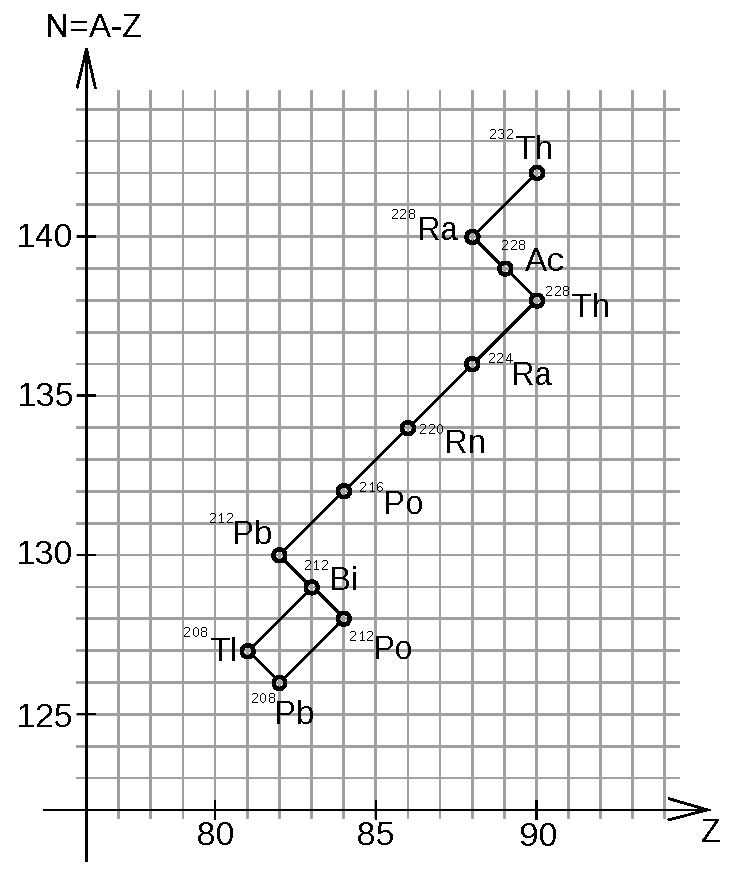
\includegraphics[width=\linewidth]{../Thorium}
    \caption{%
        Thorium-Reihe
        \parencite{thorium}
    }
    \label{fig:thorium}
    \end{subfigure}
    \hfill
    \begin{subfigure}[b]{0.48\linewidth}
    \centering
    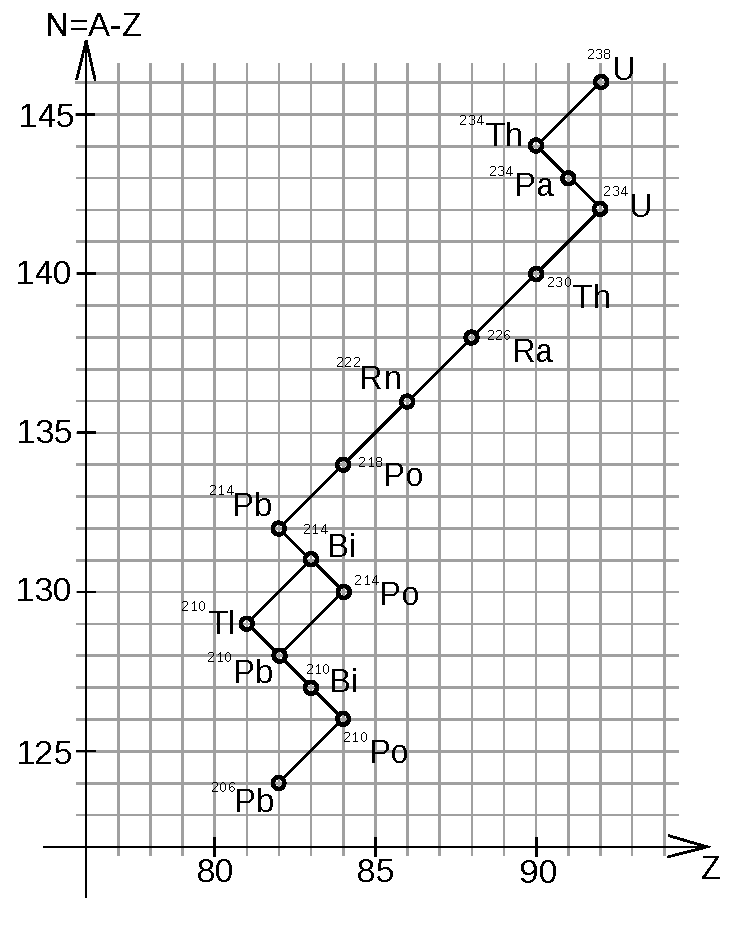
\includegraphics[width=\linewidth]{../Uran}
    \caption{%
        Uran-Radium-Reihe
        \parencite{uran}
    }
    \label{fig:uran}
    \end{subfigure}
    \caption{%
        Natürliche Zerfallsreihen
    }
    \label{fig:}
\end{figure}

$^{68}\text{Ga}$ und $^{64}\text{Cu}$ kommen nicht natürlich vor, werden aber
in der Medizin eingesetzt.



\chapter{Ergebnis}

In diesen Versuch haben wir gut sehen können, dass die Energie- und Zeitauflösung der
beiden Detektoren sehr unterschiedlich ist. Die Energiekalibrierung hat gut funktioniert. 
Deshalb lassen sich die Isotope der Bodenprobe gut bestimmen. Die identifizierten Isotope 
passen sehr gut zu dem was man erwarten würde, da ein großer Teil den
natürlichen Zerfallsreihen angehört. Die Linie des
nicht natürlich vorkommenden $^{137}\text{Cs}$-Isotops lässt sich mit dem
Unglück in Tschernobyl erklären. Sie ist immer noch deutlich erkennbar, was bei
einer Halbwertszeit von 30 Jahren auch gut möglich ist.

%%%%%%%%%%%%%%%%%%%%%%%%%%%%%%%%%%%%%%%%%%%%%%%%%%%%%%%%%%%%%%%%%%%%%%%%%%%%%%%
%                                   Anhang                                    %
%%%%%%%%%%%%%%%%%%%%%%%%%%%%%%%%%%%%%%%%%%%%%%%%%%%%%%%%%%%%%%%%%%%%%%%%%%%%%%%

\begin{appendix}


\chapter{Vorbereitungen}
\section{Energiekalibrierung}

\subsection{Szintillationsspektrometer}
\begin{figure}
    \centering
    \includegraphics[width=\plotwidth]{Sz-CO-peaks}
    \caption{%
	    Spitzen des $^{60}\text{Co}$-Spektrums aus dem NaJ(Ti)-Detektor
	    mit angepassten Gauß-Kurven
        %
    }
    \label{fig:}
\end{figure}

\begin{figure}
    \centering
    \includegraphics[width=\plotwidth]{Sz-CS-peaks}
    \caption{%
	    Spitzen des $^{137}\text{Cs}$-Spektrums aus dem NaJ(Ti)-Detektor
	    mit angepassten Gauß-Kurven
        %
    }
    \label{fig:}
\end{figure}

\begin{figure}
    \centering
    \includegraphics[width=\plotwidth]{Sz-EU-peaks}
    \caption{%
	    Spitzen des $^{152}\text{Eu}$-Spektrums aus dem NaJ(Ti)-Detektor
	    mit angepassten Gauß-Kurven
        %
    }
    \label{fig:}
\end{figure}

\begin{figure}
    \centering
    \includegraphics[width=\plotwidth]{sz_channels}
    \caption{%
	    Energiekalibrierung des NaJ(Ti)-Detektors
        %
    }
    \label{fig:sz_kanal}
\end{figure}

\subsection{Ge-Detektor}

\begin{figure}
    \centering
    \includegraphics[width=\plotwidth]{Ge_calib-peaks}
    \caption{%
	    Spitzen des $^{152}\text{Eu}$-Spektrums aus dem Ge-Detektor  mit
	    angepassten Lorentz-Kurven
    }
    \label{fig:Ge-peaks}
\end{figure}

\begin{figure}
    \centering
    \includegraphics[width=\plotwidth]{ge_channels}
    \caption{%
	    Energiekalibrierung des Ge-Detektors
        %
    }
    \label{fig:ge_kanal}
\end{figure}



\clearpage

\chapter{Langzeitmessung}

\section{Identifizieren der Isotope}\label{anhang-bodenprobe}
Auf den folgenden Abbildungen sieht man oben eine an die Daten angepasste
Lorentzkurve in dem dafür genutzten Datenbereich. In der Mitte wurden die
Spektren aus der Datenbank mit den bestpassenden Spektren überlagert und unten
diese Überlagerung nach Elementen aufgeschlüsselt.

%TODO

%< for num, first, last, kev in plot_fit_peaks >%
\begin{figure}
    \centering
    \includegraphics[width=.8\linewidth]{plot_fit_peak__<< num >>_langzeit}
    \includegraphics[width=.8\linewidth]{element_match_<< num >>_score}
    \includegraphics[width=.8\linewidth]{element_match_<< num >>_contrast}
    \caption{%
        \SI{<< kev >>}{\kilo\electronvolt}-Linie
    }
    \label{fig:}
\end{figure}
%< endfor >%

\end{appendix}

\end{document}

% vim: spell spelllang=de tw=79
